%\documentclass[12pt]{article}
%\usepackage[a4paper, margin=1in]{geometry} 
%\usepackage{graphicx} 
%\usepackage{hyperref}
%\usepackage{float}
%\usepackage{multicol}
%\usepackage{multirow}
%\usepackage[font=small, labelfont=bf]{caption}
%
%\begin{document} 

%
% BLAST
%
\subsection{BLAST}
BLAST (Basic Local Alignment Search Tool) is the most popular tool to find homologous sequences in large-scale sequence databases.

%
% Methods
%
\subsubsection*{Methods} 
\begin{itemize}
\item Generate n-grams from query sequence
\item Find n-gram hits in database
\item Expand n-gram hits to HSP
\item Increase HSP scores
\item Introducing gaps
\item Give the expect values (E-values) to HSPs
\end{itemize}

%
% N-gram hits to HSP
%
\subsubsection*{N-gram hits to HSP} 
\begin{itemize}
\item Connect multiple n-gram hits 
\item Increase HSP score
\end{itemize}

\begin{figure}[H]
  \centering
      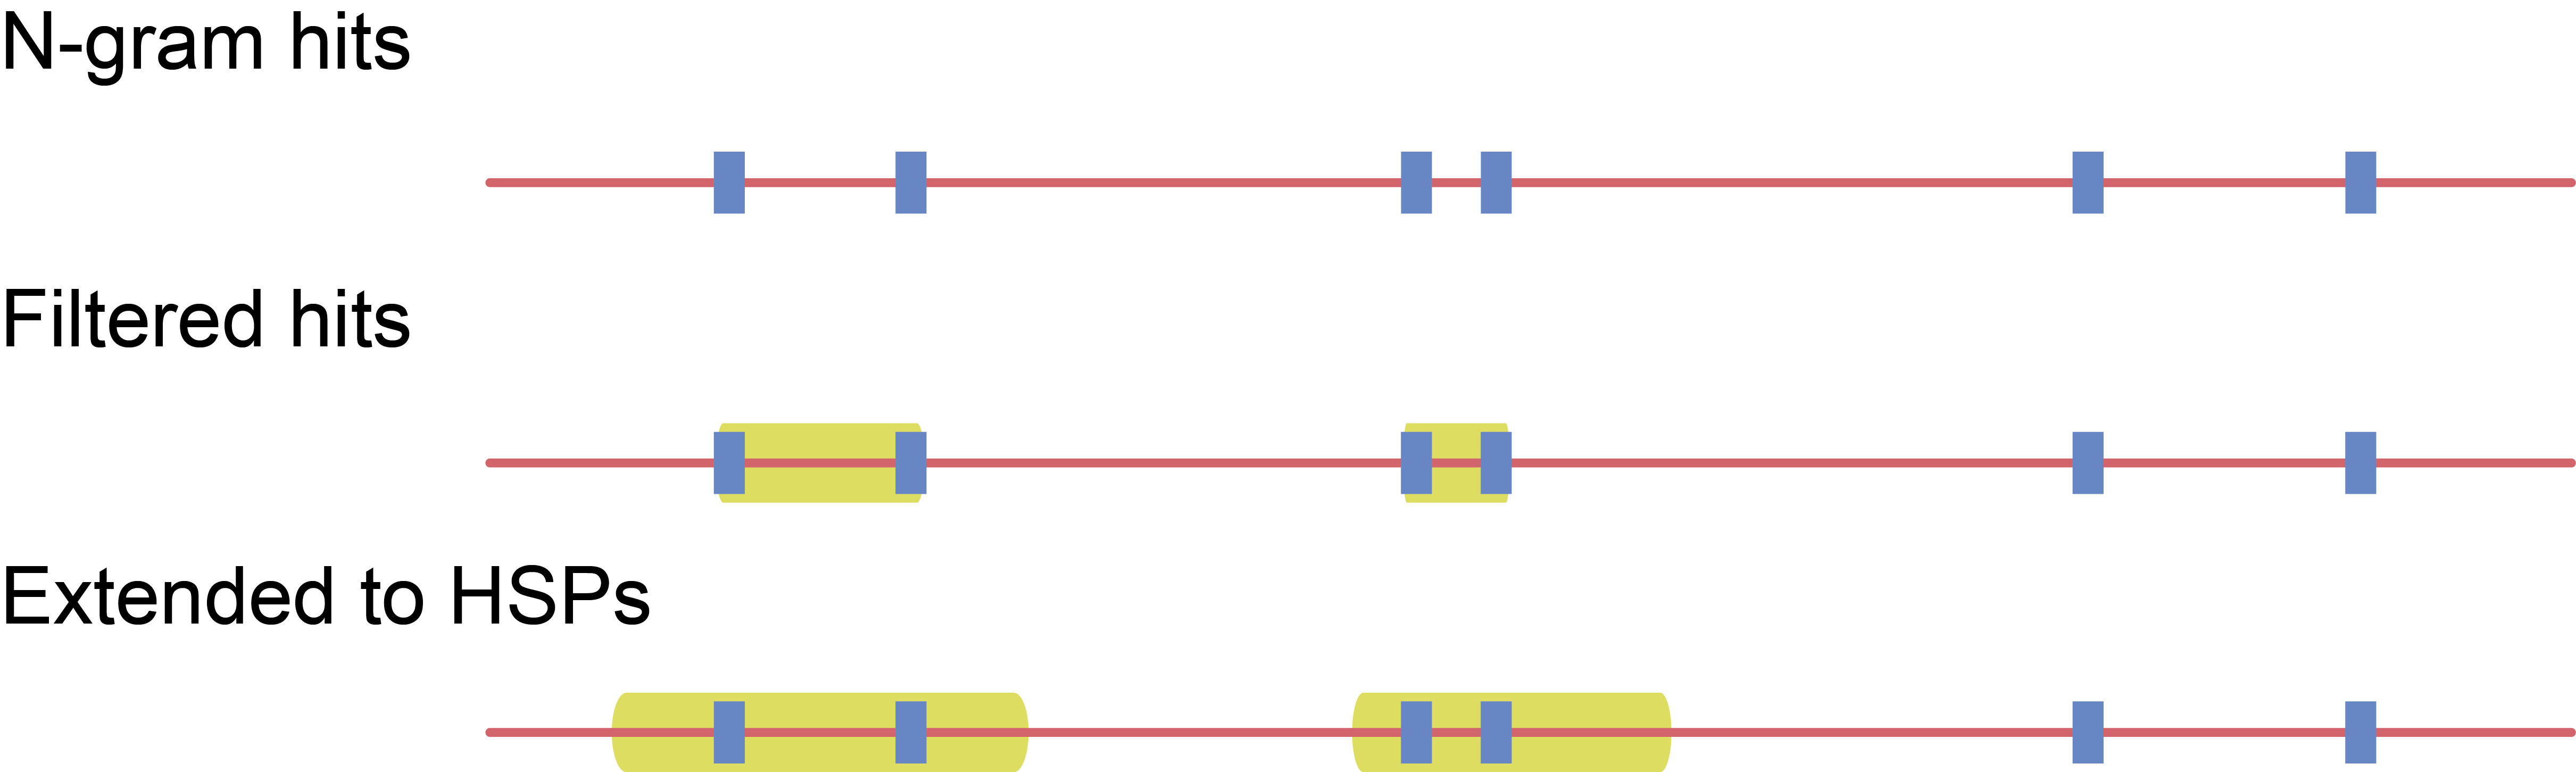
\includegraphics[width=0.75\textwidth]{fig05/extend_hsps.png}
  \caption{N-gram hits to HSPs}
\end{figure}

%
% Increase HSP score
%
\subsubsection*{Increase HSP score} 
BLAST changes the length of HSP by shortening or extending in order to increase the score.

\noindent
\textbf{Example}
\begin{figure}[H]
  \centering
      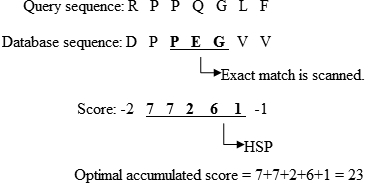
\includegraphics[width=0.45\textwidth]{fig05/extension_process.png}
  \caption{HSP extension process (source: \href{https://commons.wikimedia.org/w/index.php?curid=32912508}{DISP, Wikimedia Commons})}
\end{figure}

%
% Introducing gaps
%
\subsubsection*{Introducing gaps} 
Banded dynamic programming is used to introduce gaps to an HSP.

\begin{figure}[H]
  \centering
      
\includegraphics[width=0.25\textwidth]{fig05/banded_dp.png}
  \caption{Banded DP with the starting seed pair}
\end{figure}

%
% E-value
%
\subsubsection*{E-value} 
``The Expect value (E) is a parameter that describes the number of hits one can expect to see by chance when searching a database of a particular size'' \\ \\
-- BLAST Frequently Asked questions (\href{http://blast.ncbi.nlm.nih.gov}{http://blast.ncbi.nlm.nih.gov})

\bigskip 

%\end{document}
